
\documentclass[10pt]{article}






\usepackage[cmex10]{amsmath}
\usepackage{amscd}
\usepackage{amssymb}
\usepackage{amsthm}
\usepackage{relsize}
\usepackage{xspace}




\usepackage{tikz}
\usetikzlibrary{arrows,decorations,backgrounds,shapes}





\oddsidemargin 0.8cm
\textwidth 6.0in
\topmargin 0.0in
\textheight 20.5cm



\newtheorem{thm}{Theorem}[section]
\newtheorem{cor}[thm]{Corollary}
\newtheorem{lem}[thm]{Lemma}

\newtheorem*{lem*}{Lemma}

\theoremstyle{remark}
\newtheorem{remark}[thm]{Remark}
\newtheorem{claim}[thm]{Claim}

\theoremstyle{definition}
\newtheorem{definition}[thm]{Definition}

\theoremstyle{plain}
\newtheorem{fact}[thm]{Fact}

\newcommand{\struct}[1]{\ensuremath{\mathcal #1}}
\newcommand{\enc}[1]{\ensuremath{\mathsf{enc}\left( #1 \right)}}
\def\etal{~et~al.\ }
\newcommand{\linebrk}{\vspace{0.3cm}}

\newcommand{\logic}[1]{\textsf{\upshape\relsize{-0.5}#1}\xspace}
\newcommand{\FP}{\logic{FP}}
\newcommand{\FPC}{\logic{FP+C}}
\newcommand{\FPRK}{\logic{FP+rk}}
\newcommand{\FOL}{\logic{FO}}
\newcommand{\FOC}{\logic{FO+C}}
\newcommand{\FORK}{\logic{FO+rk}}
\newcommand{\MSO}{\logic{MSO}}
\newcommand{\INF}{\ensuremath{\logic L^\omega_{\infty\omega}}}
\newcommand{\FODTC}{\logic{DTC}}
\newcommand{\FOSTC}{\logic{STC}}
\newcommand{\FOTC}{\logic{TC}}
\newcommand{\FOrk}{\FORK}
\newcommand{\CPTCard}{\logic{PT(Card)}}

\newcommand{\ifp}{\operatorname{ifp}}
\newcommand{\tc}{\operatorname{tc}}
\newcommand{\dtc}{\operatorname{dtc}}
\newcommand{\stc}{\operatorname{stc}}
\newcommand{\rk}{\operatorname{rk}}
\newcommand{\RK}{\operatorname{RK}}
\newcommand{\free}{\operatorname{free}}
\newcommand{\spn}{\operatorname{span}}
\newcommand{\inv}{\operatorname{inv}}

\newcommand{\cclass}[1]{\ensuremath{\mathrm{#1}}\xspace}
\newcommand{\PTIME}{\cclass{PTIME}}
\newcommand{\MODL}[1]{\ensuremath{\cclass{MOD}_{#1} \, \cclass{L}}}
\newcommand{\PARITYL}{\ensuremath{\oplus \cclass{L}}}
\newcommand{\LOGSPACE}{\cclass{LOGSPACE}}

\renewcommand {\phi}{\varphi}
\renewcommand{\epsilon}{\varepsilon}
\newcommand{\isom}{\ensuremath{\cong}}
\newcommand{\GF}[1]{\ensuremath{\mathsf{GF}_{#1}}}
\newcommand{\sle}[1]{\ensuremath{\mathfrak #1}} \newcommand{\univ}[1]{\ensuremath{U \! ( \struct{#1} )}} \newcommand{\bigmid}{\;\big|\;}
\newcommand{\modout}{\!\diagup\!\!}
\newcommand{\qedd}[1]{\hfill {\scriptsize\it #1} \ensuremath{\square}}


\DeclareMathOperator{\nequiv}{\not\equiv}
\def\TODO{\textbf{TODO:} }
\def\notmodels{\mathrel|\joinrel\neq}
\def\Q{\ensuremath{\mathbb{Q}}}
\def\N{\ensuremath{\mathbb{N}}}
\def\C{\ensuremath{\mathbb{C}}}
\def\Z{\ensuremath{\mathbb{Z}}}
\def\R{\ensuremath{\mathbb{R}}}









\begin{document}

\title{Capturing Polynomial Time on Interval Graphs}


\author{Bastian Laubner\\
  {\small Institut f\"ur Informatik}\\
  {\small Humboldt-Universit\"at zu Berlin}\\
  {\small laubner@informatik.hu-berlin.de}
}

\date{}


\maketitle

\begin{abstract}
  We prove a characterization of all polynomial-time computable queries on the class of interval graphs by sentences of fixed-point logic with counting. More precisely, it is shown that on the class of unordered interval graphs, any query is polynomial-time computable if and only if it is definable in fixed-point logic with counting. This result is one of the first establishing the capturing of polynomial time on a graph class which is defined by forbidden induced subgraphs. For this, we define a canonical form of interval graphs using a type of modular decomposition, which is different from the method of tree decomposition that is used in most known capturing results for other graph classes, specifically those defined by forbidden minors. The method might also be of independent interest for its conceptual simplicity. Furthermore, it is shown that fixed-point logic with counting is not expressive enough to capture polynomial time on the classes of chordal graphs or incomparability graphs.
\end{abstract}



\section{Introduction}\label{sec:intro}

Capturing results in descriptive complexity match the expressive power of a logic with the computational power of a complexity class. The most important open question in this area is whether there exists a natural logic whose formulas precisely define those queries which are computable in polynomial time (\PTIME). While Immerman and Vardi showed in 1982 that fixed-point logic captures \PTIME under the assumption that a linear order is present in each structure (cf. Theorem \ref{thm:immermanVardi}), there is no logic which is currently believed to capture \PTIME on arbitrary unordered structures. Despite that limitation, precise capturing results for \PTIME in the unordered case can be obtained for restricted classes of structures. Since all relational structures of a fixed finite vocabulary can be encoded efficiently as simple graphs, capturing results on restricted graph classes are of particular interest in this context.

This approach has been very fruitful in the realm of graph classes defined by lists of forbidden minors. Most of these results show that \PTIME is captured by fixed-point logic with counting \FPC when restricting ourselves to one such class, such as planar graphs~\cite{gro98a}, graphs of bounded tree-width~\cite{gromar99}, or -free graphs~\cite{grohe08definable}. In fact, Grohe has recently shown that \FPC captures \PTIME on any graph class which is defined by a list of forbidden minors~\cite{grohe10fixed}.

Given such deep results for classes of minor-free graphs, it is natural to ask if similar results can be obtained for graph classes which are defined by a (finite or infinite) list of forbidden induced subgraphs. Much less is known here. For starters, it is shown in \cite{grohe09fixed-point} and in Section \ref{sec:noCaptureCompGraphs} that a general capturing result analogous to Grohe's is not possible for \FPC on subgraph-free graph classes, such as chordal graphs or graphs whose complements are comparability graphs of partial orders. These two superclasses of interval graphs are shown to be a ceiling on the structural richness of graph classes on which capturing \PTIME requires less effort than for general graphs. 
\begin{thm}\label{thm:notCaptureCompGraphs}
 \FPC fails to capture \PTIME on the class of incomparability graphs and on the class of chordal graphs.
\end{thm}




The main result in this paper is a positive one affirming that \FPC captures \PTIME on the class of interval graphs. This means that a subset  of the class of interval graphs is decidable in \PTIME if and only if there is a sentence of \FPC defining .

\begin{thm}\label{thm:captureIntGraphs}
 \FPC captures \PTIME on the class of interval graphs.
\end{thm}

The result is shown by describing an \FPC-definable canonization procedure for interval graphs, which for any interval graph constructs an isomorphic copy on an ordered domain. The capturing result then follows from the Immerman-Vardi theorem. The proof of Theorem \ref{thm:captureIntGraphs} also has a useful corollary.

\begin{cor}\label{cor:IntGraphsDefinable}
 The class of interval graphs is \FPC-definable.
\end{cor}

There has been persistent interest in the algorithmic aspects of interval graphs in the past decades, also spurred by their applicability to DNA sequencing (cf. \cite{zhang94algorithm}) and scheduling problems (cf. \cite{moehring84algorithmic}). In 1976, Booth and Lueker presented the first recognition algorithm for interval graphs~\cite{booth76testing} running in time linear in the number of vertices and edges, which they followed up by a linear-time interval graph isomorphism algorithm~\cite{lueker79linear}. These algorithms are based on a special data structure called \emph{PQ-trees}. Using so-called perfect elimination orderings, Hsu and Ma~\cite{hsu99fast} and Habib\etal~\cite{habib00lex-bfs} later presented linear-time recognition algorithms based on simpler data structures.

All these approaches have in common that they make inherent use of an underlying order of the graph, which is always available in \PTIME computations as the order in which the vertices are encoded on the worktape. Particularly, the construction of a perfect elimination ordering by lexicographic breadth-first search needs to examine the children of a vertex in some fixed order. However, such an ordering is not available when defining properties of the bare unordered graph structure by means of logic. Therefore, most of the ideas developed in these publications cannot be applied in the canonization of interval graphs in \FPC.

We note that an algorithmic implementation of our method would be inferior to the existing linear-time algorithms for interval graphs. Given that our method must rely entirely on the inherent structure of interval graphs and not on an additional ordering of the vertices, we reckon that is the price to pay for the disorder of the graph structure.

The main commonality of existing interval graph algorithms and the canonical form developed here is the construction of a \emph{modular decomposition} of the graph. Modules are subgraphs which interact with the rest of the graph in a uniform way, and they play an important algorithmic role in the construction of modular decomposition trees (cf. \cite{brandstaedt99graph}). As a by-product of the approach in this paper, we obtain a specific modular decomposition tree that is \FPC-definable. Such modular decompositions are fundamentally different from \emph{tree decompositions}, which are the ubiquitous tool of \FPC-canonization proofs for the aforementioned minor-free graph classes (cf. \cite{grohe08definable} for a survey of tree decompositions in this context). Since tree decompositions do not appear to be very useful for defining canonical forms on subgraph-free graph classes, showing the definability of modular decompositions is a contribution to the systematic study of capturing results on these graph classes.









\section{Preliminaries and notation}

We write  and  for the positive and non-negative integers, respectively. For , let  be the \emph{closed interval of integers from  to }, and let . Tuples of variables  are often denoted by  and their length by .



A binary relation  on a set  is a \emph{strict partial order} if it is irreflexive and transitive. Two elements  of a partially ordered set  are called \emph{incomparable} if neither  nor . We call  a \emph{strict weak order} if it is a strict partial order, and in addition, incomparability is an equivalence relation, i.e., whenever  is incomparable to  and  is incomparable to , then  and  are also incomparable. If  are incomparable with respect to a strict weak order , then  implies .

Finally, a \emph{(strict) linear order} is a strict partial order in which no two elements are incomparable. If  defines a strict weak order on  and  is the equivalence relation defined by incomparability, then  induces a linear order on .


\subsection{Graphs}

All graphs in this paper are assumed to be finite, simple, and undirected unless explicitly stated otherwise. Let  be a graph with vertex set  and edge set . Generally,  is viewed as a binary relation. Sometimes, we also find it convenient to view edges  as sets containing their two endpoints, as in . For isomorphic graphs  and  we write .

For  a set of vertices,  denotes the \emph{induced subgraph} of  on . The \emph{neighborhood} of a vertex , denoted , is the set of vertices adjacent to  under , \emph{including  itself}.

A subset  is called a \emph{clique} of  if  is a complete graph. A clique  of  is \emph{maximal} if it is inclusion-maximal as a clique in , i.e., if no vertex  can be added to  so that  forms a clique. Since maximal cliques are central to the constructions in this paper, they will often just be called \emph{max cliques}. \emph{Cycles} in a graph are defined in the usual way.

A graph  is a \emph{split graph} if its vertex set can be partitioned into two sets  and  so that  is a clique and  is an independent set. We write  to emphasize on the partition. Similarly, if  is a \emph{bipartite graph}, then we write  in order to emphasize that  and  are independent sets.




The main result of this paper, Theorem \ref{thm:captureIntGraphs}, is about interval graphs, which we define and discuss now. The properties of interval graphs mentioned here are based on \cite{gilmore64characterization}.

\begin{definition}[Interval graph]
Let  be a finite collection of closed intervals . The graph  defined by  has vertex set  and edge relation .  is called an \emph{interval representation} of a graph  if . A graph  is an \emph{interval graph} if there is a collection of closed intervals  which is an interval representation of .
\end{definition}

If , then  denotes the interval corresponding to vertex  in . An interval representation  for an interval graph  is called \emph{minimal} if the set  is of minimum size over all interval representations of . Any interval representation  can be converted into a minimal interval representation by removing a subset of  from all intervals in  (and then considering the remaining points in  as an initial segment of ).



If  is a minimal interval representation of , then there is an intimate connection between the max cliques of  and the sets  for . In fact, if  for some , then  forms a clique which is maximal by the minimality condition on . Conversely, if  is a max clique of , then  for some  by the minimality of , and . Thus, a connected graph  is an interval graph if and only if its max cliques can be arranged as a path so that each vertex of  is contained in consecutive max cliques. In this way, any minimal interval representation  of  induces an ordering  of 's max cliques. We call a max clique  a \emph{possible end} of  if there is a minimal interval representation  of  so that  is -minimal.

Interval graphs are a classical example of an \emph{intersection graph class} of certain objects. Intersection graphs have as vertices a collection  of these objects with an edge between  and  if and only if . Notice that any finite graph is the intersection graph of some collection of sets from , which is not the case when we restrict the allowed sets to intervals.

If  is an intersection graph class, , and  is any subset of , then  is also a member of  since it is just the intersection graph of the objects in . Any graph class  that is closed under taking induced subgraphs can also be defined by a possibly infinite list of \emph{forbidden induced subgraphs}, by taking all those graphs not in  that are minimal with respect to the relation of being an induced subgraph. A complete infinite family of forbidden induced subgraphs defining the class of interval graphs is given by Lekkerkerker and Boland in \cite{lekkerkerker62representation}.



Some further classes of graphs are important for this paper, and will be defined now.

\begin{definition}[Chordal graph]
A graph is called \emph{chordal} if all its induced cycles are of length 3.
\end{definition}

It is easy to show that every interval graph is chordal. Chordal graphs can alternatively be characterized by the property that the maximal cliques can be arranged in a forest , so that for every vertex of the graph the set of max cliques containing it is connected in  (cf. \cite{diestel06graphtheory}).



\begin{definition}[Comparability graph]
A graph  is called a \emph{comparability graph} if there exists a strict partial ordering  of its vertex set  so that  if and only if  are comparable with respect to .
\end{definition}

A graph is called an \emph{incomparability graph} if its complement is a comparability graph. It is a well-known fact that every interval graph is an incomparability graph. In fact, a graph is an interval graph if and only if it is a chordal incomparability graph \cite{gilmore64characterization, golumbic04algorithmic}.




\subsection{Logics}

We assume basic knowledge in logic, particularly of first-order logic \FOL. All structures considered in this paper are graphs , i.e., relational structures with universe  and one binary relation  which is assumed to be symmetric and irreflexive. This section will introduce the fixed-point logics \FP and \FPC. Detailed discussions of these logics can be found in \cite{ebbinghaus99finite, graedel07finite, immerman99descriptive}.

If  is a formula of some logic, we write  to indicate that the free variables of  are among . If  are vertices of a graph , then  denotes that  satisfies  if  is interpreted as  for all . Furthermore,  denotes the subset of vertices  in  for which , and similarly, .

\emph{Inflationary fixed-point logic} \FP is the extension of \FOL by a fixed-point operator with inflationary semantics, which is defined as follows. Let  be a graph, let  be a \emph{relation variable} of arity , and let  be a vector of  variables. Let  be a formula whose free variables may include  as a free relation variable and  as free (vertex) variables. For any set , let  denote the set of -tuples  for which  holds when  is interpreted as  and  is assigned to . Let the sets  be defined inductively by  and .  Since  for all , we have  for all . We call the -ary relation  the \emph{inflationary fixed-point} of  and denote it by . \FP denotes the extension of \FOL with the -operator.

In 1982, Immerman~\cite{immerman82bounds} and Vardi~\cite{vardi82complexity} showed that \FP characterizes \PTIME on classes of ordered structures\footnote{In fact, Immerman and Vardi showed this capturing result using a different fixed-point operator for \emph{least fixed points}. Inflationary and least fixed points were shown to be equivalent by Gurevich and Shelah~\cite{gurevich85fixed-point} and Kreutzer~\cite{kreutzer04equivalence}. Also, Immerman and Vardi proved the result for general relational structures with an ordering, while we only state their theorem for graphs.}.

\begin{thm}[Immerman-Vardi]\label{thm:immermanVardi}
Let  be a class of ordered graphs, i.e., graphs with an additional binary relation  which satisfies the axioms of a linear order. Then  is \PTIME-decidable if and only if there is a sentence of \FP defining .
\end{thm}

When no ordering is present, then \FP is not expressive enough to capture \PTIME; in fact, it cannot even decide the parity of the underlying vertex set's size. For the capturing result in this paper, we will also need a stronger logic which is capable of such basic counting operations.

For this, let  be a graph and let . Instead of  alone, we consider the two-sorted structure  with universe , so that  defines  on  and  is the natural linear ordering of . Notice that  is not defined for any numbers from , and also,  does not give any order on . Now we define \FP-sentences on  with the convention that all variables are implicitly typed. Thus, any variable  is either a vertex variable which ranges over  or a numeric variable which ranges over .

The connection between the vertex and the number sort is established by \emph{counting terms} of the form  where  is a vertex variable and  is a formula.  denotes the number from  of vertices  so that . \FPC is now obtained by extending \FP in the two-sorted framework with counting terms. 
We can encode numbers from  with -tuples of number variables. With the help of the fixed-point operator, we can do some meaningful arithmetic on these tuples, such as addition, multiplication, and counting the number of tuples  satisfying a formula  (cf. \cite{graedel07finite}).

With its power to handle basic arithmetic, \FPC is already more powerful than \FP on unordered graphs. Still, it is not powerful enough to capture \PTIME by a result of Cai, F\"urer and Immerman~\cite{cai92optimal}. This fact will be used in the next section to prove similar negative results for specific classes of graphs. For this, we still need the notion of a \emph{graph interpretation}, which is a restricted version of the more general concept of a syntactical interpretation.

\begin{definition}\label{def:graphInterpretation}
 An \emph{-ary graph interpretation} is a tuple  of \FOL-formulas so that  and in any graph,  defines an equivalence relation on . If  is a graph, then  denotes the graph with vertex set  and edge set .
\end{definition}


\begin{lem}[Graph Interpretations Lemma]\label{lem:graphInterpretationsLemma}
 Let  be an -ary graph interpretation. Then for any \FPC-sentence  there is a sentence  with the property that .
\end{lem}

\proof[Idea.] A proof of this fact for first-order logic can be found in \cite{ebbinghaus94mathematical}. It essentially consists in modifying occurrences of the edge relation symbol and quantification in  with the right versions of ,  and . Lemma \ref{lem:countEqClasses} below is needed in order to deal with counting quantifiers in a sensible manner. We omit the details. \qed


\subsection{\FPC-definable canonization}

Results that prove the capturing of \PTIME on a certain graph class usually do so by showing that there is a logically definable canonization mapping from the graph structure to the number sort. Theorem \ref{thm:captureIntGraphs} will also be proved in this way, showing that there is an \FPC-formula  with numeric variables  and  so that any interval graph  is isomorphic to . Since the number sort  is linearly ordered, the Immerman-Vardi Theorem \ref{thm:immermanVardi} then implies that any \PTIME-computable property of interval graphs can be defined in \FPC.

Cai, F\"urer and Immerman have observed that for graph classes which admit \FPC-definable canonization, a generic method known as the Weisfeiler-Lehman (WL) algorithm can be used to decide graph isomorphism in polynomial time (cf. \cite{cai92optimal}). Thus by Theorem \ref{thm:captureIntGraphs}, the WL algorithm also decides isomorphism of interval graphs. In the light of efficient linear-time isomorphism algorithms for interval graphs, the novelty here lies in the fact that a simple combinatorial algorithm decides interval graph isomorphism without specifically exploiting these graphs' inherent structure. The algorithm is generic in the sense that it also decides isomorphism of planar graphs, graphs of bounded treewidth, and many others.



\subsection{Basic formulas}

We finish this section by noting some basic constructions that can be expressed in \FPC. The existence of these formulas is essentially folklore, and variants of them can for example be found in \cite{graedel07finite}. These results lay the technical foundation for a higher-level description of the canonization procedure in Section \ref{sec:CapOnIntGraphs}. We omit their straight-forward proofs.

\begin{lem}[Counting equivalence classes] \label{lem:countEqClasses}
Suppose  is an \FPC-definable equivalence relation on -tuples of , and let  be an \FPC-formula with . Assume that  has at most  equivalence classes. Then there is an \FPC-counting term giving the number of equivalence classes  of  such that  for some . \qed
\end{lem}

\proof The idea is to construct the sum slicewise for each cardinality of equivalence classes first, which gives us control over the number of classes rather than the number of elements in these classes.  Let  be number variables. Define the relation  to hold if  is contained in a -equivalence class of size  which contains some element making  true. Using the fixed-point operator, it is then easy to define relation  for  from  to . Then  is the desired counting term. \qed

Let  be a tuple of numeric variables and let  be some formula. Using the ordering on the number sort and fixing ,  can be considered a 0-1-string of truth values of length . If  is a tuple of elements so that the string defined by  is the lexicographically least of all such strings, then  is called the \emph{lexicographic leader}. Observe that such  need not be unique. Lexicographic leaders are used to break ties during the inductive definition of a graph's ordered canonical form.

\begin{lem}[Lexicographic leader] \label{lem:lexLeaderDefable}
Let  be a tuple of variables taking values in  and let  be a tuple of number variables. Suppose  is an \FPC-formula and  is an \FPC-definable equivalence relation on . Then there is an \FPC-formula  so that for any ,  is the lexicographic leader among the relations . \qed
\end{lem}

\proof To start, there is a \FOL-sentence  so that  holds if and only if  is lexicographically smaller or equal to . Now  is given by

\qed


Finally, we will repeatedly encounter the situation where the disjoint union of given graphs has to be defined in a canonical way. If  are (ordered) graphs in lexicographically ascending order, then we define their disjoint union  on  so that  is order isomorphic to  for all . It is easy to see that  is uniquely well-defined, and we call it the \emph{lexicographic disjoint union} of . The following lemma says that lexicographic disjoint unions are \FPC-definable.


\begin{lem}\label{lem:lexDisjUnionDefable}
Suppose  is an \FPC-definable equivalence relation on  and let ,  be \FPC-formulas with number variables  defining graphs  on the numeric sort for each . Furthermore, assume that  whenever , and that .  Then there is an \FPC-formula  defining on  the lexicographic disjoint union of the lexicographic leaders of 's equivalence classes. \qed
\end{lem}

\proof Let  be the strict weak order on 's equivalence classes induced by the strict weak order on the classes' respective lexicographic -leader. Using Lemma \ref{lem:lexLeaderDefable}, it is easy to define , using elements from  to identify equivalence classes. Using the fixed point-operator, define  inductively starting with the -least elements, saving those elements  from equivalence classes that have already been considered in a relation . In each step, find the -least elements  in  which are not in , calculate the number  of equivalence classes contained in , and then expand  by  copies of  (which is the same for any ). \qed



\section{Non-capturing results}\label{sec:noCaptureCompGraphs}

This section contains some negative results of \FPC not capturing \PTIME on a number of graph classes. In particular, this will be shown for bipartite graphs (Theorem \ref{thm:notCapOnBipGraphs}) using a simple construction and the machinery of graph interpretations (see Definition \ref{def:graphInterpretation}). Theorem \ref{thm:notCaptureCompGraphs} will then follow. We note that Theorem \ref{thm:notCapOnBipGraphs} has previously been obtained by Dawar and Richerby~\cite{dawar07power}. However, the method used here is more widely applicable and allows for stronger conclusions (see Remark \ref{rem:strongerConclusion}).

The results in this section are all based on the following theorem due to Cai, F\"urer, and Immerman~\cite{cai92optimal}.

\begin{fact} \label{fact:CFI}
 There is a \PTIME-decidable property  of graphs of degree  which is not \FPC-definable.
\end{fact}

For any graph , the \emph{incidence graph}  is defined by  and .  is bipartite and it is straightforward to define a graph interpretation  so that for any graph  it holds that . Furthermore, given a graph , it is a simple -computation to uniquely reconstruct  from . Also, since the two parts of a bipartite graph can be found in linear time, it is clear how to decide whether a given graph  is isomorphic to  for some graph .

\begin{thm} \label{thm:notCapOnBipGraphs}
 \FPC does not capture \PTIME on the class of bipartite graphs.
\end{thm}

\proof Recall the \PTIME-decidable query  from Fact \ref{fact:CFI} and let  for some . By the remarks above,  is \PTIME-decidable.

So suppose that \FPC captures \PTIME on the class of bipartite graphs. Then there is an \FPC-sentence  such that for every bipartite graph  it holds that  if and only if . By an application of the Graph Interpretations Lemma \ref{lem:graphInterpretationsLemma} we then obtain a sentence  so that  if and only if . Thus,  defines , contradicting Fact \ref{fact:CFI}.\qed


Theorem \ref{thm:notCaptureCompGraphs} is now a simple corollary of the following Lemma.


\begin{lem}\label{lem:bipGraphIsCompGraph}
Every bipartite graph  is a comparability graph.
\end{lem}

\proof A suitable partial order  on  is defined by letting  if and only if , , and .\qed

\begin{cor}
 \FPC does not capture \PTIME on the class of incomparability graphs.\qed
\end{cor}


This tells us that being a comparability or incomparability graph alone is not sufficient for a graph  to be uniformly \FPC-canonizable. Section \ref{sec:CapOnIntGraphs}, however, is going to show that this is possible if  is both chordal \emph{and} an incomparability graph, i.e., an interval graph. In a way, this is not simply a corollary of a capturing result on a larger class of graphs, as it is shown now that \FPC does not capture \PTIME on the class of chordal graphs, either. The construction is due to Grohe~\cite{grohe09fixed-point}.


For any graph , the \emph{split incidence graph}  is given by  and . Notice that  differs from  only by the fact that all former vertices  form a clique in . 
Given the similarity of  and , the analysis for split incidence graphs is completely analogous to the one for incidence graphs above. In particular, the class  is \PTIME-decidable and given a split graph , the graph  for which  can be reconstructed in \PTIME if such  exists. Also, there is a graph interpretation  so that for any graph : . The proof of the following theorem is then clear, and the subsequent lemmas complete the analysis for chordal graphs.

\begin{thm}\FPC does not capture \PTIME on split graphs.\qed
\end{thm}


\begin{lem}
Every split graph  is chordal.\qed
\end{lem}


\begin{cor}[Grohe~\cite{grohe09fixed-point}]
 \FPC does not capture \PTIME on the class of chordal graphs.\qed
\end{cor}

\begin{remark} \label{rem:strongerConclusion}
In fact, the proofs here admit even stronger conclusions: any \emph{regular logic} (cf. \cite{ebbinghaus94mathematical}) captures \PTIME on the class of comparability graphs (respectively chordal graphs) if and only if it captures \PTIME on the class of all graphs.
\end{remark}

Let us conclude this section by noting some non-capturing results for further intersection graph classes. A -interval graph is the intersection graph of sets which are the union of  intervals. By a result of Griggs and West \cite{griggs79extremal}, any graph of maximum degree 3 is a -interval graph, so Fact \ref{fact:CFI} directly implies that \FPC does not capture \PTIME on -interval graphs for . In \cite{Uehara08simple}, Uehara gives a construction that implies such a non-capturing result for intersection graphs of axis-parallel line segments in the plane. It follows that \FPC does not capture \PTIME on boxicity- graphs for , where a boxicity- graph is the intersection graph of axis-parallel boxes in  and the boxicity- graphs are just the interval graphs.







\section{Capturing \PTIME on interval graphs}\label{sec:CapOnIntGraphs}

The goal of this section is to prove Theorem \ref{thm:captureIntGraphs} by canonization. We will exhibit a numeric \FPC-formula  so that for any interval graph ,  defines a graph on the numeric sort of \FPC which is isomorphic to . The canonization essentially consists of finding the lexicographic leader among all possible interval representations of . For this, as discussed above, it is enough to bring the maximal cliques of  in the right linear order. The first lemma shows that the maximal cliques of  are \FOL-definable.

\begin{lem} \label{lem:maxCliquesDefable}
Let  be an interval graph and let  be a maximal clique of . Then there are vertices , not necessarily distinct, such that .
\end{lem}

This is fairly intuitive. Consider the following minimal interval representation of a graph .

\begin{center}
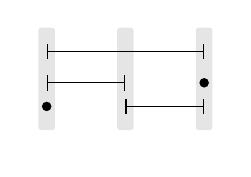
\begin{tikzpicture}
 \foreach \x in {1,...,3}
{
 \fill[xshift=\x cm-1cm,rounded corners=1pt,fill=gray!20!white] (-3pt,-.3cm) rectangle (3pt,1cm);
 \draw[xshift=\x cm-1cm] (0,-.3cm) node[anchor=north] {\small };
}

 \filldraw (0,0) node[anchor=east] {\small } circle (1.5pt)
	(2,.3) node[anchor=west] {\small } circle (1.5pt);
 \draw[|-|] (0,.3) -- (1,.3) node[midway,above] {\small };
 \draw[|-|] (0,.7) -- (2,.7) node[near start,above] {\small };
 \draw[|-|] (1,0) -- (2,0) node[midway,above] {\small };
\end{tikzpicture}
\end{center}

Max cliques  and  are precisely the neighborhoods of vertices  and , respectively. The vertex pairs , , and  all define max clique , and similarly three different vertex pairs define max clique . Max clique  is not the neighborhood of any single vertex, but it is uniquely defined by .


\proof[Proof of Lemma \ref{lem:maxCliquesDefable}]  Let  be a minimal interval representation of . First assume that  is the -least maximal clique. The lemma is trivial if  is the only maximal clique of , otherwise let  be 's -successor. Since  there is , and  is the only maximal clique of  that  is contained in (as  is contained in -consecutive max cliques). Hence, . A symmetric argument holds if  is the -greatest maximal clique. Now assume that  is neither -least nor maximal and let  be 's immediate -predecessor and successor, respectively. There exist  and , and we claim that . In fact, since any vertex in  is contained both in  and , we have . Now let  and write . Let  be the (unique) integer such that . Then  implies , and  implies . Thus,  and hence , which proves the claim. \qed


Now, whether or not a vertex pair  defines a max clique is easily definable in \FOL, as is the equivalence relation on  of vertex pairs defining the same max clique. Lemma \ref{lem:maxCliquesDefable} tells us that \emph{all} max cliques can be defined by such vertex pairs. For any , let the \emph{span of }, denoted , be the number of max cliques of  that  is contained in. Since equivalence classes can be counted by Lemma \ref{lem:countEqClasses},  is \FPC-definable on the class of interval graphs by a counting term with  as a free vertex variable.

Generally representing max cliques by pairs of variables  allows us to treat max cliques as first-class objects that can be quantified over. For reasons of conceptual simplicity, the syntactic overhead which is necessary for working with this representation will not be made explicit in the remainder of this section.

\subsection{Extracting information about the order of the maximal cliques}
Now that we are able to handle maximal cliques, we would like to simply pick an end of the interval graph  and work with the order which this choice induces on the rest of the maximal cliques. Of course, the choice of an end does not necessarily impose a linear order on the maximal cliques. However, the following recursive procedure turns out to recover all the information about the order of the max cliques induced by choosing an end of .

Let  be the set of maximal cliques of an interval graph  and let . The binary relation  is defined recursively on the elements of  as follows:


The following interval representation of a graph  illustrates this definition.

\begin{center}
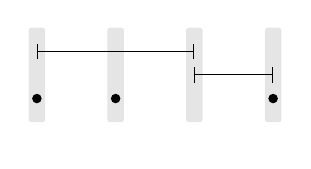
\begin{tikzpicture}
 \foreach \x/\xtext in {1/M,2/C,3/D,4/X}
{
 \fill[xshift=\x cm-1cm,rounded corners=1pt,fill=gray!20!white] (-3pt,-.3cm) rectangle (3pt,.9cm);
\draw[xshift=\x cm-1cm] (0,-.3cm) node[anchor=north] {\small };
}

 \filldraw (0,0) circle (1.5pt)
	(1,0) circle (1.5pt)
	(3,0) circle (1.5pt);
\draw[|-|] (0,.6) -- (2,.6) node[near start,above] {\small };
\draw[|-|] (2,.3) -- (3,.3) node[midway,above] {\small };	

\end{tikzpicture}
\end{center}

Suppose we have picked max clique , then  and  since  and  by the initialization step. In a second step, it is determined that  since  and . So in this example,  actually turns out to be a strict linear order on the max cliques of . This is not the case in general, but  will still be useful when  is a possible end of . The definition of  seems natural to me for the task of ordering the max cliques of an interval graphs. However, I am not aware of it appearing previously anywhere in the literature.

It is readily seen how to define  using the inflationary fixed-point operator, where maximal cliques are defined by pairs of vertices from .

\begin{remark} \label{rem:alreadySTC}
 In fact,  can already be defined using a \emph{symmetric transitive closure} operator as follows: define an edge relation on  by connecting  and  if  follows from  by one application of (\ref{eqn:indDef}). Inspection of (\ref{eqn:indDef}) shows that this edge relation is symmetric, hence the graph is undirected. Now  holds if and only if  is reachable from  for some max clique . This observation is used in \cite{koebler10interval} to show that canonical forms of interval graphs can be computed using only logarithmic space.
\end{remark}


The following lemmas prove important properties of . We say that a binary relation  on a set  is \emph{asymmetric}\index{asymmetric relation} if  implies  for all . In particular, asymmetric relations are irreflexive.

\begin{lem} \label{lem:antisymImpTransitive}
If  is asymmetric, then it is transitive. Thus, if  is asymmetric, then it is a strict partial order.
\end{lem}

\proof By a derivation chain of length  we mean a finite sequence , , ,  such that  and for each , the relation  follows from  by one application of (\ref{eqn:indDef}). Clearly, whenever it holds that  there is a derivation chain that has  as its last element.

So assume that  is asymmetric. Suppose  and let a derivation chain  of length  be given for . The proof is by induction on . If , then  and  holds. For the inductive step, suppose  and consider the second to last element  in the derivation chain. There are two cases:
\begin{itemize}
\item  and there is a vertex : By induction it holds that . Now if we had , the fact that  would imply , which contradicts asymmetry of . Hence,  and one more application of (\ref{eqn:indDef}) yields .
\item  and there is a vertex : If , then we immediately get . If , then . Thus we can derive  where the left derivation chain has length . By induction,  follows.\qed
\end{itemize}


\begin{lem}\label{lem:moduleImpIncomparable}
Let  be a set of max cliques with . Suppose that for all  and any  it holds that . Then the max cliques in  are mutually incomparable with respect to .
\end{lem}

\proof Suppose for contradiction that there are  with . Let , , ,  be a derivation chain for  as in the proof of Lemma \ref{lem:antisymImpTransitive}. Since , , and , there is a largest index  so that either  or  is not contained in .

If , then  and  and it holds that . Consequently, , contradicting the assumption of the lemma. Similarly, if , then  and  and it holds that . Thus, , again a contradiction.\qed


In fact, there is a converse to Lemma \ref{lem:moduleImpIncomparable} when the set of -incomparable max cliques is maximal.



\begin{lem} \label{lem:sameIntersection}
Suppose  is a max clique of  and  is a maximal set of -incomparable max cliques. Let . Then  for all .
\end{lem}

\proof We say that a max clique  \emph{splits} a set of max cliques  if there are  so that . If in addition to splitting ,  is also -comparable to all the elements in , then either  or  and one application of (\ref{eqn:indDef}) implies that  and  are comparable.

Suppose for contradiction that there is  splitting .
We greedily grow a list of max cliques  with the property that  splits the set .
The list  is complete when no further max clique splits the set .

Suppose that . For any  we have  for all , so Lemma \ref{lem:moduleImpIncomparable} implies that the max cliques in  are -incomparable. However, this is impossible since we assumed  to be maximal. Therefore, .


Now let  be a shortest list of max cliques from  so that  and each  splits .

\begin{claim}\label{claim:auxLemSameIntersection}
For all ,  for all .
\end{claim}
\proof[Proof of Claim \ref{claim:auxLemSameIntersection}] Consider  and suppose that there is  with . As  splits , there must be some  such that . But then  already splits , so by eliminating  we could make the list shorter.

Inductively, suppose that the claim holds for all , but not for . Then there are  such that , so  already splits . Removing  from the list gives us a shorter list in which  still splits  for all  because of our inductive assumption. As we assumed our list to be shortest, this concludes the inductive step. \qedd{Claim \ref{claim:auxLemSameIntersection}}




We now argue once again inductively backwards down the list  with the goal of showing that  is -comparable to all max cliques in . Certainly, this is true for  and . Assume that  is comparable to all max cliques in  for . Since  for all  by Claim \ref{claim:auxLemSameIntersection}, it follows that  is comparable to all max cliques in .

Now  is comparable to all max cliques in . Since  splits , there are  so that , contradicting our assumption that the max cliques in  are -incomparable. Therefore we conclude that there is no  splitting .\qed



Lemma \ref{lem:sameIntersection} says that incomparable max cliques interact with the rest of  in a uniform way. Let us make this notion more precise. A \emph{module} of  is a set  so that for any vertex ,  is either completely connected or completely disconnected to . In other words, for all  and all  it holds that . The next drawing illustrates the occurrence of a module in an interval graph.

\begin{center}
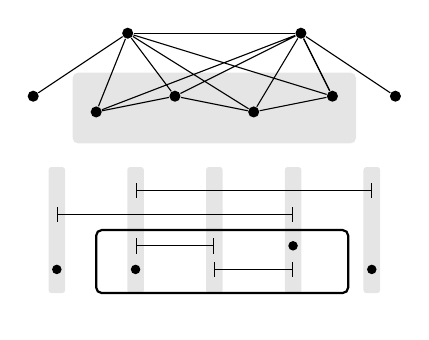
\begin{tikzpicture}[v/.style={circle,fill,inner sep=0pt,minimum size=4pt}]
 \foreach \x in {1,...,5}
{
 \fill[xshift=\x cm-1cm,rounded corners=1pt,fill=gray!20!white] (-3pt,-.3cm) rectangle (3pt,1.3cm);
\draw[xshift=\x cm-1cm] (0,-.3cm) node[anchor=north] {\small };
}

 \draw[thick,rounded corners=2pt] (.5,-.3cm) rectangle (3.7,.5) node[anchor=north east] {};

 \filldraw (0,0) circle (1.5pt)
	(1,0) circle (1.5pt)
	(3,.3) circle (1.5pt)
	(4,0) circle (1.5pt);

 \draw[|-|] (0,.7) -- (3,.7);
 \draw[|-|] (1,1) -- (4,1);
 \draw[|-|] (1,.3) -- (2,.3);
 \draw[|-|] (2,0) -- (3,0);	


 \def\x{-1}
 \def\y{2};
 \fill[gray!20!white,rounded corners=2pt] (\x+1.2,\y+.5) rectangle (\x+4.8,\y-.4) node[anchor=south east,black] {};

 \node[v] (1) at (\x+.7,\y+.2) {};
 \node[v] (2) at (\x+1.9,\y+1) {};
 \node[v] (3) at (\x+1.5,\y) {};
 \node[v] (4) at (\x+2.5,\y+.2) {};
 \node[v] (5) at (\x+3.5,\y) {};
 \node[v] (6) at (\x+4.5,\y+.2) {};
 \node[v] (7) at (\x+4.1,\y+1) {};
 \node[v] (8) at (\x+5.3,\y+.2) {};


\draw (1) -- (2) -- (3) -- (4) -- (5) -- (6) -- (7) -- (8);
\draw (2) -- (4) -- (7) -- (5) -- (2) -- (6) -- (7) -- (3);
\draw (2) -- (7);


\end{tikzpicture}
\end{center}



\begin{cor}\label{cor:incompImpModule}
Suppose  is a max clique of  so that  is a strict partial order and  is a maximal set of incomparable max cliques. Then
\begin{itemize}
 \item  is a module of , and
 \item .
\end{itemize}
\end{cor}

\proof Let  and  and suppose that , but . There is a max clique  with , but , and since  we must have . By the definition of ,  is also contained in some max clique . Finally, let  be some max clique in  containing , so . Thus, , contradicting Lemma \ref{lem:sameIntersection}.

For the second statement, let . If , then clearly . But if , then it is contained in some , and by Lemma \ref{lem:sameIntersection}  must also be contained in all max cliques in . Thus, , proving the statement. \qed

This characterization of the modules occurring when defining the relations  will be central in the canonization procedure of . There is another corollary of Lemma \ref{lem:sameIntersection} which proves that  has a particularly nice structure.


\begin{cor}\label{cor:strictOrderImpWeakOrder}
 If  is a max clique of  so that  is a strict partial order, then  is a strict weak order.
\end{cor}

\proof We need to prove that -incomparability is a transitive relation of 's max cliques. So let  and  be incomparable pairs with respect to . Let  and  be maximal sets of incomparables containing  and , respectively. By Lemma \ref{lem:sameIntersection}, we have  for every  and . As  Lemma \ref{lem:moduleImpIncomparable} implies that the max cliques in  are -incomparable, so in particular  and  are incomparable with respect to .\qed



At this point, let us put the pieces together and show that picking an arbitrary max clique  as an end of  and defining  is a useful way to obtain information about the structure of .

\begin{lem} \label{lem:partialOrderEqEnd}
Let  be a max clique of an interval graph . Then  is a strict weak order if and only if  is a possible end of .
\end{lem}

\proof If  is a possible end of , then let  be a minimal interval representation of  which has  as its first clique. Let  be the linear order  induces on the max cliques of . In order to show asymmetry it is enough to observe that, as relations, we have . It is readily verified that this holds true of the initialization step in the recursive definition of , and that whenever max cliques  satisfy (\ref{eqn:indDef}) with  replaced by , then it must hold that . This shows asymmetry, and by Lemma \ref{lem:antisymImpTransitive} and Corollary \ref{cor:strictOrderImpWeakOrder}  is a strict weak order.

Conversely, suppose  is a strict weak order. The first aim is to turn  into a linear order. Let  be a maximal set of incomparable max cliques, and recall the set . Since  is an interval graph, we can pick an interval representation  for . The set of max cliques of  is given by , and since  is a module,  for any  from . Thus,  induces a linear order  on the elements of . Now let  if and only if , or  for some maximal set of incomparables  and . This is a strict linear order since  is a strict weak order. We claim that  is an ordering of the max cliques which is isomorphic to the linear order induced by some interval representation of . This will imply that  is a possible end of .

In order to prove the claim, it is enough to show that each vertex  is contained in consecutive max cliques. Suppose for contradiction that there are max cliques  and  is contained in  and , but not in . Certainly, this cannot be the case if  are incomparable with respect to , so assume without loss of generality that . Now, since , (\ref{eqn:indDef}) implies that , which contradicts the asymmetry of . \qed

\begin{remark} \label{remark:doesntWorkGenerally}
 The recursive definition of  and Lemma \ref{lem:antisymImpTransitive} through Corollary \ref{cor:strictOrderImpWeakOrder} do not depend on  being an interval graph. However, the proof of Lemma \ref{lem:partialOrderEqEnd} shows that  only turns out to be a partial order if the max cliques can be brought into a linear order, modulo the occurrence of modules. In particular, defining  in a general chordal graph does not yield any useful information if the graph's tree decomposition into max cliques requires a tree vertex of degree 3 or more, which is the case for all chordal graphs which are not interval graphs.
\end{remark}


\subsection{Canonizing when  is a linear order}\label{subsec:canLinOrder}

Since  is \FP-definable for any max clique , and since asymmetry of  is \FOL-definable, Lemma \ref{lem:partialOrderEqEnd} gives us a way to define possible ends of interval graphs in \FP. Moreover, if  is a possible end of , then  contains precisely the ordering imposed on the max cliques of  by the choice of  as the first clique.

First, suppose that  is an interval graph and  is a linear order on the max cliques which is induced by an interval representation of . Define the binary relation  on the vertices of  as follows. For , let  be the -least max clique of  containing . Then let


It is readily verified that  is a strict weak order on , and if  are incomparable, then . Now it is easy to canonize : if  denotes the equivalence class of vertices incomparable to , then  is represented by the numbers from the interval , where  is the number of vertices which are strictly -smaller than . Since all vertices in  have precisely the same neighbors in  and  forms a clique, it is also clear how to define the edge relation on the number sort.

Now if  is any interval graph and  is a possible end, we can still define an ordering for those vertices that are not contained in a module. Let  be the equivalence relation on  for which  if and only if  or there is a nonsingular maximal set of incomparables  with respect to  so that . Denote the equivalence class of  under  by , and define the edge relation  of the graph  by  s.t. . It follows directly from the definition of  that if  is a max clique which is -comparable to all other max cliques in , then all  are in singleton equivalence classes . If  is a nonsingular maximal set of incomparables, then there is precisely one max clique  in  which contains all the equivalence classes associated with , i.e., . Thus  induces a strict linear order on the max cliques of . In fact, this shows that  is an interval graph with a valid interval representation induced by . 










\subsection{Canonizing general interval graphs} \label{subsec:generalIntGraphs}
What is left is to deal with the sets  coming from maximal sets of incomparables. Let . For each  define  as the set of vertices of the connected component of  which intersects  (if non-empty). Notice that  is a max clique of . Finally, let  be the set of those  for which defining  in  yields a strict partial order of 's max cliques.

It is immediate from Corollary \ref{cor:incompImpModule} that for any maximal set of incomparable max cliques , . In this situation, for any , the set  defines a component of , and  if and only if  is a possible end of (one of the components of) . This gives us enough structure to perform canonization.





\proof[Proof of Theorem \ref{thm:captureIntGraphs}] We define the relation  inductively, where  and  are number variables.  will be an isomorphic copy of  on the numeric sort. To this end, start defining  for all , then for all , and so on, up to all .

Suppose we want to define  for , then first compute the strict weak order  on the interval graph . Consider any nonsingular maximal set of incomparables  and let . Let  be a list of the components of  and let  be such a component. By the above remarks, there exist at least two  so that  and .

Notice that by the definitions of  and , we have  and therefore all  with  have already been defined. Let  be the equivalence relation on  defined by . Using Lemma \ref{lem:lexDisjUnionDefable}, we obtain the lexicographic disjoint union  of the lexicographic leaders of 's equivalence classes.


Finally, let  be the strict partial order on  defined above. Let  be the list of non-singular equivalence classes of . Each  is associated with a unique maximal set of incomparables , and  as sets. We aim at canonizing  using , inserting the graph defined by  in place of each . Here is how: each  is represented by the interval , where  is the number of vertices in equivalence classes strictly -smaller than . Since all vertices in  have the same neighbors in all of , it is clear how to define the edge relation between  and . If  is not a singleton set, then  for some  and the edge relation on  is given by .




It is clear from the construction that . Also,  can be defined in \FPC for all  using a fixed point-operator iterating  from  to . Finally, let  be the lexicographic disjoint union of the lexicographic leaders canonizing the components of , each of which is defined by some . Then , which concludes the canonization of .\qed




\proof[Proof of Corollary \ref{cor:IntGraphsDefinable}] 
We claim that for the recognition of interval graphs, it is enough to check that (a) every edge of the graph  is contained in some max clique which is defined by the joint neighborhood of some pair of vertices and (b) the canonization procedure as described in Section \ref{sec:CapOnIntGraphs} succeeds to produce a graph of the same size on the number sort. 

Certainly, any interval graph satisfies both conditions by the results in this paper. Conversely, assume that  satisfies these conditions, and let  be the ordered graph defined by the canonization procedure. We can choose a bijection  by breaking all ties during the definition of  arbritrarily. We claim that  is an isomorphism between  and . Let  and suppose . Since the sets of max cliques respectively containing  and  are disjoint, at no point during the canonization procedure there is an edge defined between numbers corresponding to  and , and hence . If , however, then  are both contained in some definable max clique  which is forced to appear in the relations  defined by (\ref{eqn:indDef}). It is easy to see then that also , and hence  is an isomorphism. Finally, observe that any graph defined by the canonization procedure is an interval graph.








\section{Conclusion}

We have proved that the class of interval graphs admits \FPC-definable canonization. Thus, \FPC captures \PTIME on the class of interval graphs, which was shown not to be the case for any of the two obvious superclasses of interval graphs: chordal graphs and incomparability graphs. The result also implies that the combinatorial Weisfeiler-Lehman algorithm solves the isomorphism problem for interval graphs.


As noted in Remark \ref{rem:alreadySTC}, the methods in this paper can be used to define \LOGSPACE-computable canonical forms for interval graphs (cf. \cite{koebler10interval}). The \FPC-canonization of the modular decomposition tree from Section \ref{subsec:generalIntGraphs} is then replaced by Lindell's \LOGSPACE-tree canonization algorithm~\cite{lindell92logspace}. This implies that the set of logspace computable intrinsic properties of interval graphs is recursively enumerable. However, \LOGSPACE is not captured by first-order logic with the symmetric transitive closure operator: any rooted tree is converted into an interval graph by connecting each vertex to all its descendants. Arguing as in Section \ref{sec:noCaptureCompGraphs}, such a capturing result would imply an analogous capturing result on trees, which is ruled out by the work of Etessami and Immerman~\cite{etessami95tree}.


Among the graph classes considered in this paper, the only class whose status is not settled with respect to \FPC-canonization is the class of chordal comparability graphs. While it appears that the methods employed for chordal incomparability graphs here do not carry over (see Remark \ref{remark:doesntWorkGenerally}), I believe I have found a different solution, which will be contained in the journal version of this paper.

So far, little is known about logics capturing complexity classes on classes of graphs which are defined by a (finite or infinite) list of forbidden induced subgraphs. This paper makes a contribution in this direction. It seems that chordal graphs, even though they do not admit \FPC-canonization themselves, can often be handled effectively in fixed-point logic as soon as additional properties are satisfied (being a line graph, incomparability or comparability graph). It would be instructive to unify these properties. In this context, I would also like to point to Grohe's conjecture~\cite{grohe09fixed-point} that \FPC captures \PTIME on the class of claw-free chordal graphs.



\section*{Acknowledgement}
I would like to thank Martin Grohe for bringing the question of capturing \PTIME on interval graphs to my attention and for helpful discussions on the subject.


\bibliographystyle{plain}
\bibliography{references}





\end{document}
